\begin{titlepage}
 \newgeometry{margin=2cm}
 
    \centering
    
    \begin{figure}
    \centering
    \begin{subfigure}{.5\textwidth}
      \centering
      
\includegraphics[width=.7\linewidth, left]{images/images_front_page/EPFL_logo.png}
    \end{subfigure}%
    \begin{subfigure}{.5\textwidth}
      \centering
      
\includegraphics[width=.7\linewidth, right]{images/images_front_page/ESL_logo.png}
    \end{subfigure}
    
    \end{figure}

    \vspace{2cm}
    
    \textsc{\Large École Polytechnique Fédérale de Lausanne}
    \\ [1cm]
    \textbf{\textsc{\LARGE Semester Project}}
    \\ [1cm]
    {\Large DOOM in HEEP: }
    \\
    {\Large Implementation of the classic DOOM game on a fully in-house ASIC}
    \\ [0.75cm]
    {\large By Ismael Tobias Frei}
    \\ [1cm]
    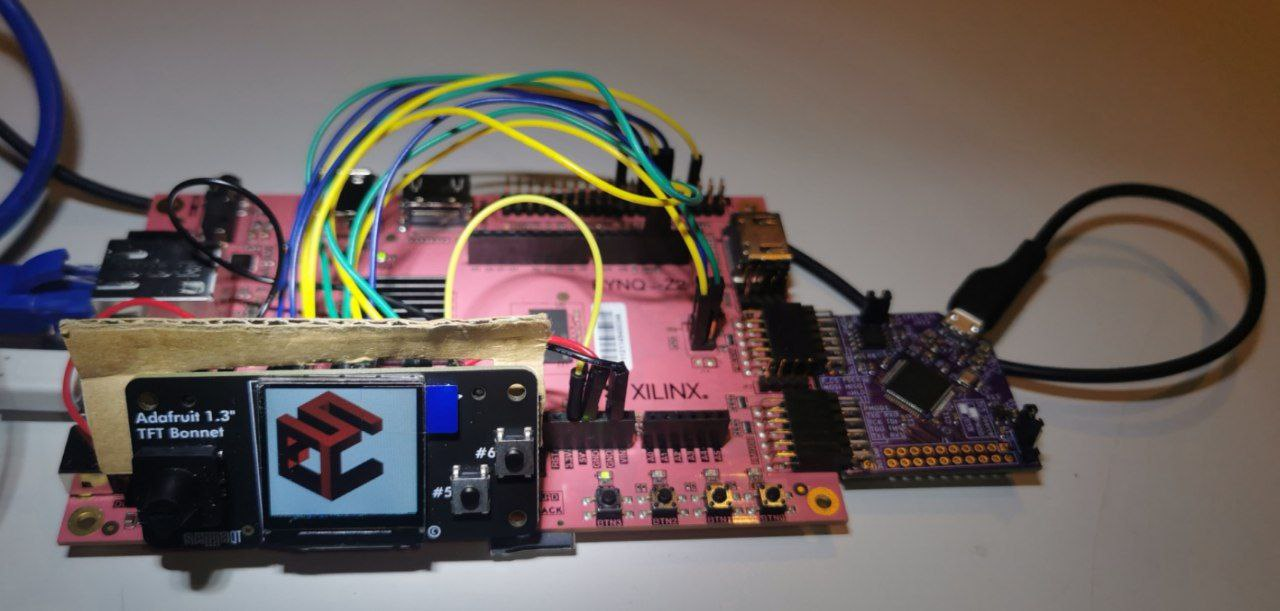
\includegraphics[width=0.8\linewidth]{images/FPGA_ESL_LOGO.jpg}
    \\[1cm]
    
    \begin{multicols}{2}
    
    \flushleft
    
    \textsc{Project Advisor:}
    \\
    Prof. David Atienza
    \\ [0.25cm]
    \textsc{Project Supervisors:}
    \\
    Dr. Jose Miranda and Dr. Miguel Peon Quiros
    
    \flushright
    
    STI IEL ESL
    \\
    ELG 130 (Bâtiment ELG)
    \\
    Station 11
    \\
    CH-1015 Lausanne
    \\
    \today
    
    \end{multicols}
\end{titlepage}